\documentclass[10pt,conference,compsocconf]{IEEEtran}

\usepackage{hyperref}
\usepackage{graphicx}	% For figure environment
\usepackage{amsmath}
%%%%%%%%%%%%%%%%%%%%%%%%%%%%%%%%%%%%%%%%%%%%%%%%%%%%%%%%%%%%%
% Some tools
% Includes a figure
% The first parameter is the label, which is also the name of the figure
%   with or without the extension (e.g., .eps, .fig, .png, .gif, etc.)
%   IF NO EXTENSION IS GIVEN, LaTeX will look for the most appropriate one.
%   This means that if a DVI (or PS) is being produced, it will look for
%   an eps. If a PDF is being produced, it will look for nearly anything
%   else (gif, jpg, png, et cetera). Because of this, when I generate figures
%   I typically generate an eps and a png to allow me the most flexibility
%   when rendering my document.
% The second parameter is the width of the figure normalized to column width
%   (e.g. 0.5 for half a column, 0.75 for 75% of the column)
% The third parameter is the caption.
\newcommand{\scalefig}[4]{
  \begin{figure}[ht!]
    % Requires \usepackage{graphicx}
    \centering
    \includegraphics[width=#2\columnwidth]{pics/#1}
 \caption{#3}
    \label{#4}
  \end{figure}}
  
  \newcommand{\doublefig}[5]{
  \begin{figure}[ht!]
    % Requires \usepackage{graphicx}
    \centering
    \includegraphics[width=#3\columnwidth]{../pics/#1}\hfill
    \includegraphics[width=#3\columnwidth]{../pics/#2}
 \caption{#4}
    \label{#5}
  \end{figure}}

% \mathbf
\newcommand{\m}[1]{\mathbf{#1}}
\newcommand{\xx}{\mathbf{x}}
\newcommand{\xt}{\mathbf{x}^T}
\newcommand{\yy}{\mathbf{y}}
\newcommand{\ww}{\mathbf{w}}
\newcommand{\XX}{\mathbf{X}}
 
\newcommand{\Lagr}{\mathcal{L}}
\newcommand{\Lmse}{\Lagr_{MSE}}

% argmin
\newcommand{\argmin}[1]{\underset{#1}{\operatorname{argmin}}}
\newcommand{\argmax}[1]{\underset{#1}{\operatorname{argmax}}}
\newcommand{\mmin}[1]{\underset{#1}{\operatorname{min}}}
\newcommand{\mmax}[1]{\underset{#1}{\operatorname{max}}}

\newcommand*\colvec[3][]{
    \begin{pmatrix}\ifx\relax#1\relax\else#1\\\fi#2\\#3\end{pmatrix}
}


\begin{document}
\title{Project 1: Higgs Boson}

\author{
  Gael Moccand, Pascal Bienz\\
  gael.moccand@gmail.com, pascal.bienz@gmail.com\\
  \textit{Machine Learning Course, EPFL}
}

\maketitle

\begin{abstract}
At CERN, the direct observation of Higgs bosons is impossible due to their short life. Instead, one can determinate whether a proton collision generates a Higgs boson by analysing the decay. A good way to process this huge amount of data and create a prediction model is to use machine learning techniques. In this work we present how we build a model that combines a least squares regression and a Ridge regularization in order to best predict whether a given set of data is due to the creation of a Higgs boson.
\end{abstract}

\section{Introduction}
The Higgs boson is an elementary particle discovered at the Large Hadron Collider at CERN in 2013. In order to produce it, physicists accelerate protons and make them collide at high speeds. In some rare cases, the collision generates a Higgs boson. A major problem that arises when scientists want to observe the particle is that its life is very short. Indeed, a Higgs boson quickly decays into other particles. For that reason, it is observed indirectly by looking at the outputs of the decay. However, this process can become tricky because a Higgs boson's decay signature can be very much alike another particle's signature.\\
In this paper, a machine learning method that efficiently estimates the likelihood that a given measurement is due to a Higgs boson or some other particles is presented. It combines a least squares method augmented with a polynomial basis along with a Ridge regularization.\\
Two specific data sets are used to optimize the method. The first set $S_{t}$ is called the training set and contains $N=250000$ observations. It is used to develop the model. The second set $S_{v}$ is the validation set and has 568238 events. These data are used to validate the model and make sure that we the model does not overfit the data of $S_t$. In both sets, the events are characterized by 30 features. Among them, 13 are "raw" quantities about the bunch collision as measured by the detector and 17 are "derived" quantities computed from the raw features, which were selected by the physicists. Finally, let's point out that in some cases the variables of some entries are not available. In order to handle the missing data, it is primordial to apply a preprocessing stage.

\section{Methodology}
Before digging into prediction methods, it is beneficial to handle the data. The preprocessing is key and impacts the prediction. For instance, a scatter plot matrix of each features can be useful to select or drop some features. In our case, a basic standardization by subtracting the mean and dividing by the standard deviation is applied to the input data. Furthermore, the missing value are replaced by the mean of the corresponding feature, which is better than a value which has no signification. This will be referred to as simple preprocessing.  In a second phase, the positive data are replaced by the log of their inverse, i.e. $\log\left(\frac{1}{1+x}\right)$ before the standardization. Taking the log is a common technique. In this case, it makes sure that all the values are negative. This will be referred to as complex preprocessing.\\
To predict the nature of the measurement, we need to find a function that best approximates the output $\yy$ with the given inputs $\xx$
$$
y_n \approx f(\mathbf{x_n}) \ \forall n.
$$
A common choice is to use a linear regression, i.e.
$$
f(\mathbf{x_n}) = w_0 +  \xx_n^T\begin{pmatrix} w_1 \\ \vdots\\ w_D \end{pmatrix} =: \tilde{\xx}_n^T \ww
$$
where $\ww = (w_0 \ldots w_D)$ are the parameters of the models. Note that we add a tilde over the input vector to indicate that it contains an offset term.\\
A cost function is needed to estimate how well the model does. Again, a common choice is to use the Mean Square Error (MSE):
$$
\Lmse(\ww) := \frac 1N \sum_{n=1}^N \left( y_n -f(\xx_n) \right)^2
$$
As a starting point, it has been decided to chose a simple least squares regression  to compute $\ww$ directly. The parameters are given by the following expression:
$$
\ww^* = (\XX^T\XX)^{-1}\XX^T\yy
$$
where $\yy = \begin{bmatrix}y_1 \\ y_2 \\ \vdots \\y_N \end{bmatrix}$ and $\XX = \begin{bmatrix}x_{11} & x_{12} & \hdots & x_{1D} \\ x_{21} & x_{22} & \hdots & x_{2D} \\ \vdots & \vdots & \ddots & \vdots \\ x_{N1} & x_{N2} & \hdots & x_{ND} \end{bmatrix}$.
Linear models are inherently not very rich. A way to increase their representational power  it boost the inputs by adding a polynomial basis $\phi(\xx_n)$ of arbitrary degree $M$.
%$$
%\phi(\xx_n) = \begin{bmatrix} 1 & x_{n1} & x_{n1}^2 & \hdots & x_{n1}^M \\ 1& x_{n2} & x_{n2}^2 & \hdots & x_{n2}^M \\ \vdots & \vdots & \vdots & \ddots & \vdots \\ 1& x_{nD} & x_{nD}^2 & \hdots & x_{nD}^M \end{bmatrix}.
%$$
We then fit a linear model to the extended feature vector:
$$
y_n \approx \phi(\xx_n)^T\ww.
$$
Unfortunately, this tuning has a negative effect: overfitting. Regularization is a
way to mitigate this undesirable behavior by penalizing the model with a parameter $\Omega(\ww)$. The optimization problem becomes
\begin{equation}\label{eq:ridge}
\argmin{\ww} \ \Lagr(\ww) + \Omega(\ww).
\end{equation}
The Ridge regularization $\Omega(\ww) = \lambda || \ww ||_2^2$ is a natural choice and it penalizes the large model weights $w_i$. The solution of Eq.\ref{eq:ridge} is
$$
\ww^* = (\XX^T \XX + \lambda' I)^{-1} \XX^T \yy, \ \text{where} \ \lambda' = 2\lambda N.
$$


\section{Results}
For each prediction methods, the training set is split in 2 random subsets. The first one has 3/4 of the data and is used as a proper training set whereas the rest goes into a testing set to avoid overfitting.\\
As a baseline, a simple least together with a polynomial basis with different degrees and a simple preprocessing is used. As it can be seen on Fig.\ref{fig:cross_validation_least_poly}, it is obvious that the polynomial basis does not bring much. However, not every polynomial basis can be used because some basis lead to an unsolvable solution, that's the reason why some points are missing on the figure.
\scalefig{cross_validation_least_poly}{1}{MSE w.r.t polynomial degree for direct least squares method}{fig:cross_validation_least_poly}.\\
Secondly, the Ridge regularization is added. The first task is to tune the hyperparameter $\lambda'$. It is found by cross validation that a value of $\lambda' = 0.0001$ yields better predictions.\\
Finally, when a complex preprocessing (log of inverse) is used, along with a least squares and a Ridge regularization, it yields the Fig.\ref{fig:bestfig}. It shows that an order of 8 is optimal because a higher degree clearly overfits the testing set.
\scalefig{MINIMUM_cross_validation_Ridge_poly_00001_with_log}{1}{MSE w.r.t polynomial degree for least squares and Ridge regularization ($\lambda' = 0.0001$) method}{fig:bestfig}.\\
A summary of the results can be found in table \ref{tab:results}.
Note that selecting raw or the derived features only gives a lower score than taking into consideration both types, even if there is information redundancy by taking both types. 
\begin{table} [htbp]
  \centering
  \begin{tabular}[c]{|l|l|}
    \hline
    Method & Test error\\
    \hline
    Simple preproc. + LS + $M=2$ &0.8019\\
    Simple preproc. + LS + Ridge & 0.8252\\
    Complex preproc. + LS + Ridge $M=8$ & \textbf{0.7467}\\
    \hline
  \end{tabular}
  \caption{Test errors of different prediction methods.}
  \label{tab:results}
\end{table}

\section{Discussion}
There are few things that can probably be improved in order to get better prediction. Firstly MSE is not a good cost function when outliers are present which is the case here. One should thus look for another cost function. Then, least squares is a pretty basic model. The next step would be to use a logistic regression instead. However, we could not manage to make it converge.\\
Regarding preprocessing, an improvement would be to weight the features independently instead of having them equally weighted. Moreover, there is a feature which only has integer numbers. A possible improvement would be not to feed it to the polynomial basis and use this feature directly. Unfortunately, this trick has not shown much improvement on the final score. Finally, when the preprocessing changed from simple to complex, the whole optimization process should be done again to guarantee the best prediction with the appropriate hyperparameters.

\section{Summary}
In this work we have shown that one can have a fairly good prediction using simple machine learning techniques like the least squares regression and the ridge regularization as long as one takes care of handling the data properly. We have also highlighted the fact that in the field of machine learning, one should be careful and that some intuition that seem good a priori yield worse prediction.%

%\begin{figure}[tbp]
%  \centering
%  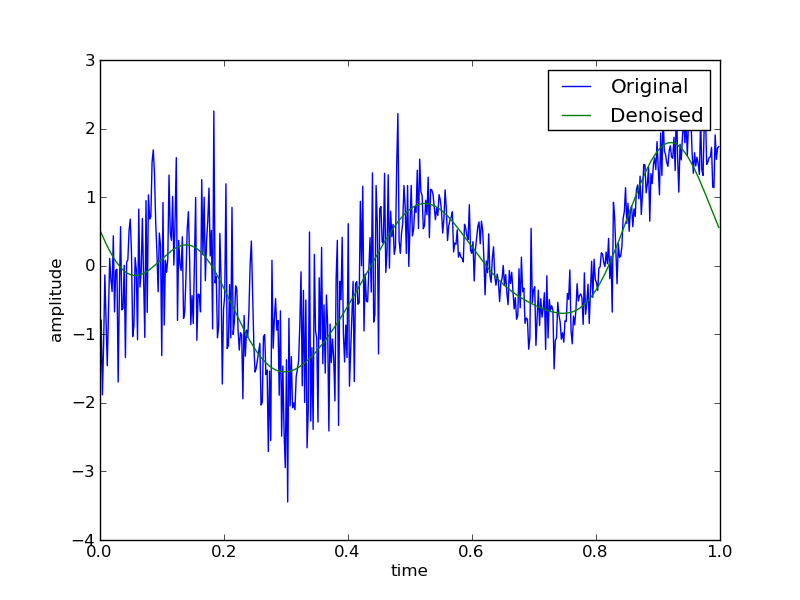
\includegraphics[width=\columnwidth]{denoised_signal_1d}
%  \caption{Signal compression and denoising using the Fourier basis.}
%  \vspace{-3mm}
%  \label{fig:denoise-fourier}
%\end{figure}
%\begin{figure}[htbp]
%  \centering
%  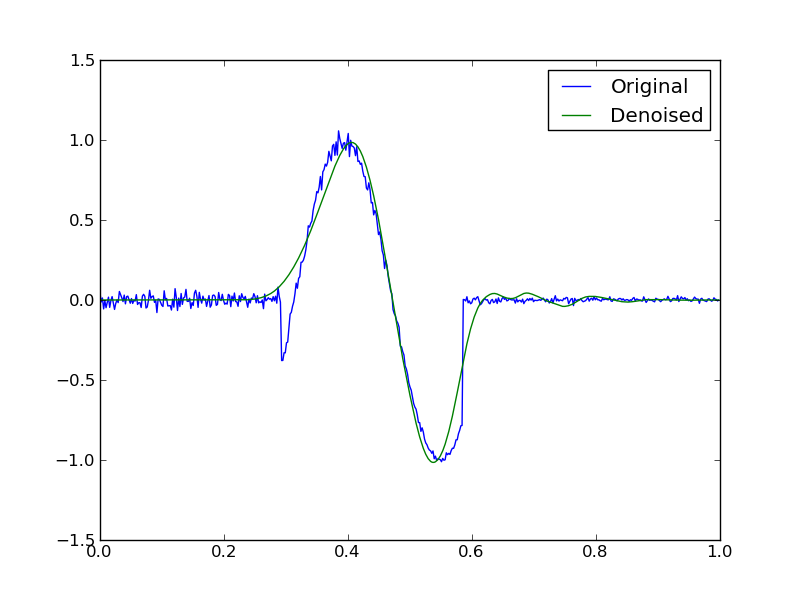
\includegraphics[width=\columnwidth]{local_wdenoised_1d}
%  \vspace{-3mm}
%  \caption{Signal compression and denoising using the Daubechies wavelet basis.}
%  \label{fig:denoise-wavelet}
%\end{figure}


%\begin{table*}[htbp]
%  \centering
%  \begin{tabular}[c]{|l||l|l|l|}
%    \hline
%    Basis&Support&Suitable signals&Unsuitable signals\\
%    \hline
%    Fourier&global&sine like&localized\\
%    wavelet&local&localized&sine like\\
%    \hline
%  \end{tabular}
%  \caption{Characteristics of Fourier and wavelet basis.}
%  \label{tab:fourier-wavelet}
%\end{table*}

%\section*{Acknowledgements}
%The author thanks Christian Sigg for his careful reading and helpful
%suggestions.

\bibliographystyle{IEEEtran}
\bibliography{literature}

\end{document}
